\documentclass{article}
\usepackage{listings}
\usepackage{graphicx}
\usepackage[slovene]{babel}
\usepackage{color}
\usepackage{amsmath}
\usepackage[usenames,dvipsnames]{xcolor}
\usepackage[hidelinks]{hyperref}
\usepackage{subcaption}
\usepackage{float}
\usepackage{rotating} 
\usepackage{hyperref}
\usepackage{caption}
\usepackage{siunitx}
\graphicspath{{./images/}}

\setlength{\parindent}{0pt}

\begin{document}

\title{Matematično-fizikalni praktikum \\[3mm] \large Naloga 8}
\author{Luka Papež}
\date{21.\ december 2024}

\begin{center}
    
\includegraphics[width=8cm]{logo-fmf.png}
\end{center}

{
    \let\newpage\relax
    \maketitle
}

\maketitle
\newpage
\section{Naloga}
Določi nekaj najnižjih lastnih funkcij in lastnih
vrednosti za
neskončno in končno potencialno jamo z diferenčno metodo in metodo streljanja, lahko pa poskusiš še iterativno in  s kakšno drugo metodo. 
Problem končne jame je s strelsko metodo le trivialna posplošitev
problema neskončne jame: spremeni se le robni pogoj pri $x=a/2$,
ki ima zaradi zahteve po zveznosti in zvezni odvedljivosti valovne
funkcije zdaj obliko $c_1\psi(a/2) + c_2\psi'(a/2) = 0$. 
Alternativno, lahko pri končni jami problem obrnemo in začnemo daleč stran, kjer je funkcija 
(in odvod le-te) skoraj nič, ter poskušamo zadeti  pogoj (soda,liha funkcija) v izhodišču. Preveri,
kaj je bolje (bolj stabilno, natančno)!
Kaj ima pri diferenčni metodi večjo vlogo pri napaki:
končna natančnost diference, s katero aproksimiramo drugi odvod,
ali zrnatost intervala (končna razsežnost matrike, ki jo
diagonaliziramo)?
\section{Uvod}

Pri robnem problemu lastnih vrednosti poznamo diferencialno enačbo
in nekaj robnih pogojev (običajno vsaj toliko, kolikor je red enačbe)
Za rešitev problema moramo v splošnem v enem zamahu določiti
tako (lastne) funkcije, ki ustrezajo danim robnim pogojem,
kot (lastne) vrednosti, ki skupaj zadoščajo diferencialni enačbi.
Reševanje robnih problemov je zato lahko bistveno bolj zapleteno
kot integracija začetnih problemov.


Numerično bomo reševali stacionarno Schr\"odingerjevo enačbo
\begin{equation*}
-\frac{\hbar^2}{2m}\,\Dd[2]{\psi}{x} + V(x)\psi = E\psi  
\end{equation*}
za neskončno potencialno jamo ($V(-a/2 < x < a/2)=0$ 
in $V(|x|\ge a/2)\to\infty$) ter za končno potencialno jamo
($V(|x|\ge a/2)=V_0$), za kateri poznamo analitične rešitve;
glej Strnad, {\sl Fizika II\/}.  Dva značilna pristopa, diferenčna
metoda in strelska metoda, nas bosta pripravila na resnejše probleme,
za katere analitičnih rešitev ne poznamo.

Pri {\sl diferenčni metodi\/} razdelimo interval
$[-a/2,a/2]$ na $N$ točk ($x_i = -a/2 + ia/N$) in prepišemo drugi
krajevni odvod v drugo diferenco, tako da ima brezdimenzijska enačba obliko
\begin{equation*}
\frac{\psi_{i-1} - 2\psi_i + \psi_{i+1}}{h^2} + E\psi_i = 0  
\end{equation*}
oziroma
\begin{equation*}
\psi_{i-1} - (2-\lambda)\psi_i + \psi_{i+1} = 0 \>,  
\end{equation*}
kjer je $\lambda=Eh^2=k^2h^2$.  Diskretizirati je treba tudi robna
pogoja pri $x=-a/2$ in $x=a/2$, ki sta v splošnem (in tudi
pri končni jami) mešanega tipa,
\begin{align*}
c_1 \psi_0 + c_2 \frac{\psi_1 - \psi_{-1}}{2h} =& 0 \>, \\
d_1 \psi_N + d_2 \frac{\psi_{N+1} - \psi_{N-1}}{2h} =& 0 \>,
\end{align*}
medtem ko sta pri neskončni jami preprostejša, $\psi_0=\psi_N=0$.
V primerih potencialnih jam tako dobimo tridiagonalni sistem $N$
oziroma $N-1$ linearnih enačb
\begin{equation*}
A \underline{\psi} = \lambda \underline{\psi}   
\end{equation*}
za lastne vektorje $\underline{\psi}$ in lastne vrednosti $\lambda$,
ki ga rešujemo z diagonalizacijo.  

\smallskip

Pri {\sl strelski metodi\/} začnemo s ``kosinusnim'' začetnim pogojem
v izhodišču $\psi(0)=1$, $\psi'(0)=0$ ali ``sinusnim'' pogojem
$\psi(0)=0$, $\psi'(0)=1$, nato pa z nekim izbranim $E$ diferencialno
enačbo s poljubno integracijsko shemo (npr.~RK4) integriramo do roba
$x=a/2$ in tam preverimo, ali je izpolnjen drugi robni pogoj, $\psi(a/2)=0$.
Vrednost $E$ spreminjamo tako dolgo, dokler robni pogoj ni izpolnjen do
zahtevane natančnosti, in tako dobimo sode in lihe rešitve enačbe
skupaj z ustreznimi lastnimi vrednostmi energije.
\section{Rešitev}
\subsection{Neskončna potencialna jama}
V prvem delu rešitve robnega problema lastnih vrednosti smo poiskali rešitve neskončne poencialne jame. Da lažje primerjamo naše rezultate si najprej oglejmo analitično rešitev. Rešujemo Schr{\"o}dingerjevo enačbo
\begin{equation}
	\frac{\hbar^2}{2m}\frac{\partial^2\psi}{\partial x^2} = (V - E)\psi\text{,}
\end{equation}
kjer nas zanima območje brez potenciala $V=0$, saj je v območju neskončnega potenciala delca ni. Temu tudi sledijo robni pogoji $\psi(0)=\psi(a)=0$. Lastne energije sistema so
\begin{equation}
	E_n=\frac{\hbar^2\pi^2}{2ma^2}n^2
\end{equation}
in lastne funkcije
\begin{equation}
	\psi_n(x)=\sqrt{\frac{2}{a}}\sin{\frac{n\pi x}{a}}\text{.}
\end{equation}
Za naše nadaljnje reševanje bomo postavili konstante na ena $\frac{\hbar}{2m}=1$ in $a=1$. Za numerično reševanje si pogledamo strelsko metodo. Pri tej moramo biti previdni, saj podana metoda implementira iskanje natančnosti odvoda, da se čim bolj prilagodi robnim pogojem. To nam sicer ustreza a se moramo zavedati, da v resnici iščemo lastne energije in moramo biti zato zmerni s toleranco. 
Oglejmo si odstopanje desnega robnega pogoja v odvisnosti od različnih energij.
\begin{figure}[H]
	\centering
	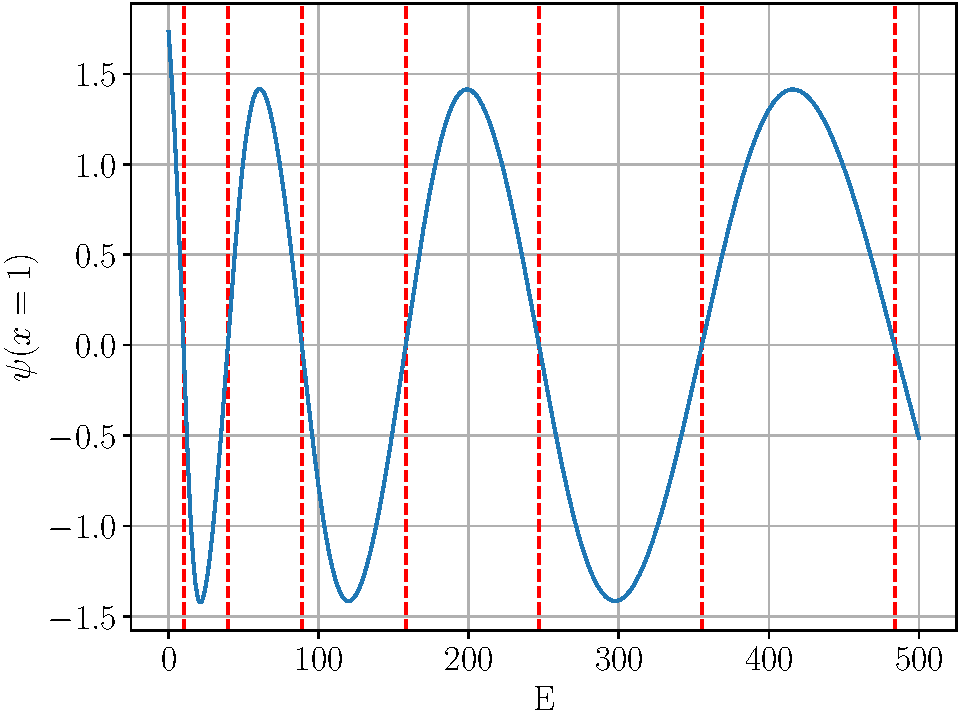
\includegraphics[width=0.7\textwidth]{diff.pdf}
	\caption{Ujemanje desnega robnega pogoja v odvisnosti od energije}
\end{figure}
Opazimo oscilacijo okrog 0, kar se ujema z našim teoretičnim znanjem. Vrednosti, kjer je $\phi(x=1) = 0$ se namreč ujema z robnim pogojem in je v drugih besedah rešitev našega problema. Poiščimo te vrednosti s preprostim algoritmom iskanja spremembe predznaka med zaporednimi točkami. Narišimo izračunane lastne funkcije.
\begin{figure}[H]
	\centering
	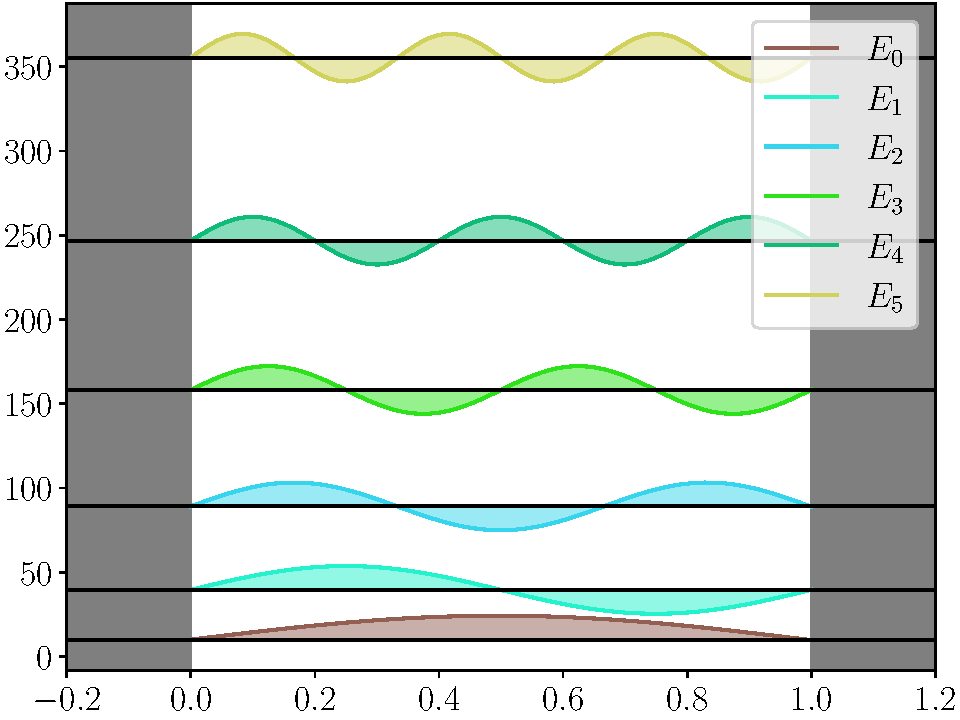
\includegraphics[width=0.7\textwidth]{eigen.pdf}
	\caption{Prvih 5 lastnih funkcij neskončne potencialne jame pomnoženih z 10}
\end{figure}
Dobljene lastne funkcije vizualno izpolnjujejo robne pogoje in se tudi ujemajo s pričakovanimi analitičnimi rezultati. Zanimala pa bi nas tudi bolj natančna primerjava, zato uporabimo metodo bisekcije, da poiščemo natančne ničle in njihove funkcije. Preden si pogledamo primerjavo se ustavimo še pri diferenčni metodi. 
Za diferenčno metodo sistem enačb $\frac{-2 \psi_i + \psi{i-1} + \psi_{i+1}}{h^2} + E\psi_{i} = 0$(za vsako točko na intervalu ena enačba) uporabimo, da sestavimo matriko. Pri tem hkrati že upoštevamo robne pogoje, da je valovna funkcija v robnih točkah enaka 0. Tako rešujemo nam že dobro poznan problem diagonalizacije. Ker je naša matrika očitno tridiagonalna, je najboljša izbira za izračun funkcije iz knjižnica `scipy`, ki je specializirana za računanje takih matrik.
\begin{figure}[H]
    \centering
    \begin{subfigure}[b]{0.49\textwidth}
        \centering
        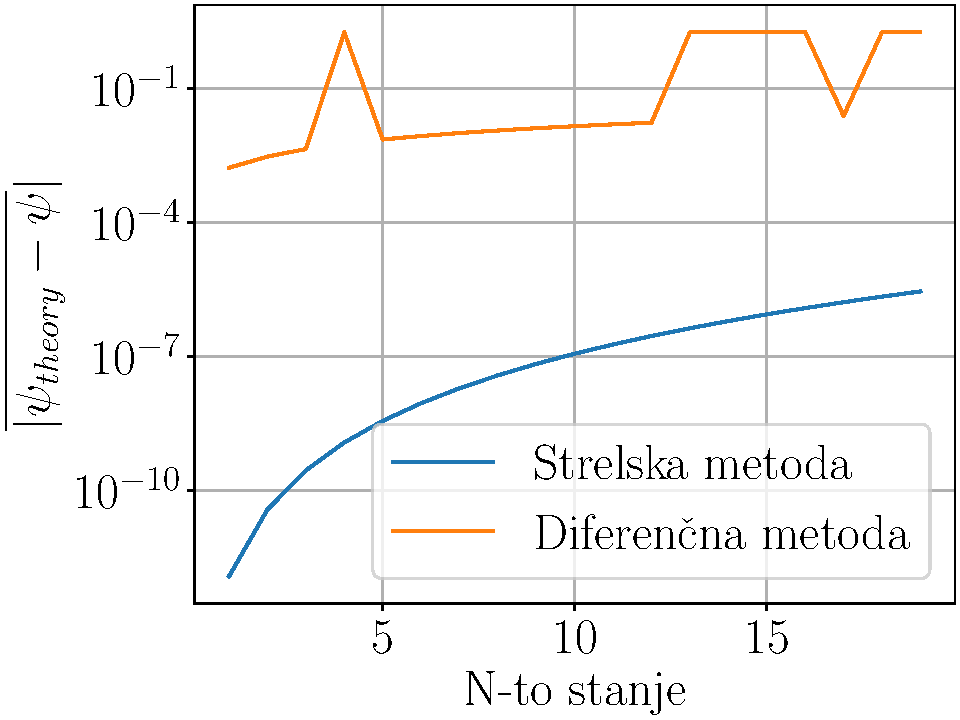
\includegraphics[width=\textwidth]{errstates.pdf}
		\caption{Natančnost N-te lastne funkcije}
    \end{subfigure}
    \hfill
    \begin{subfigure}[b]{0.49\textwidth}
        \centering
		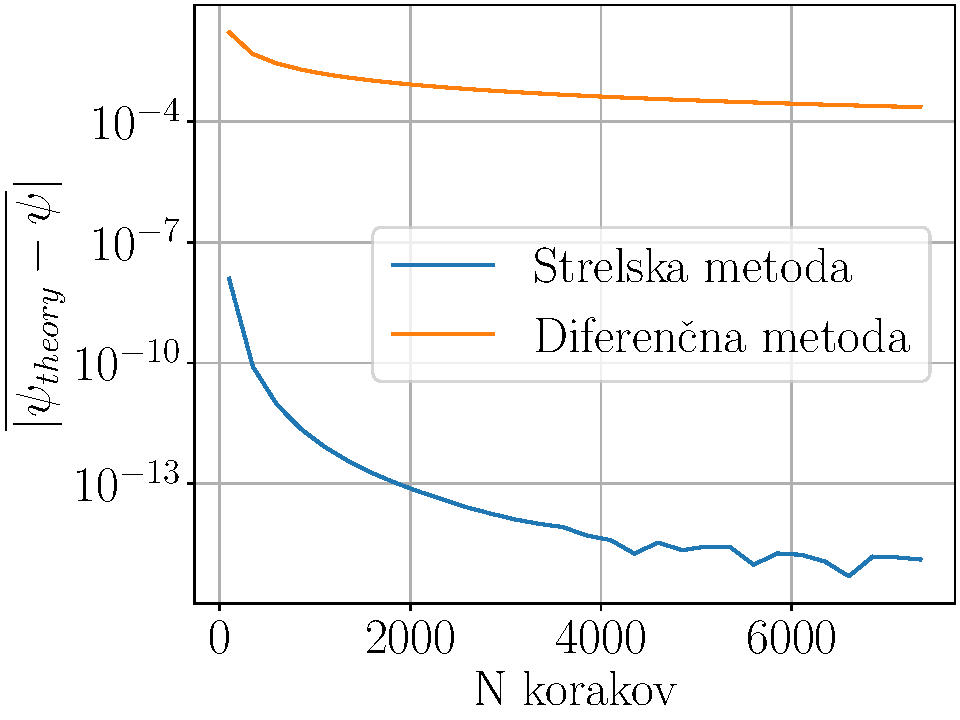
\includegraphics[width=\textwidth]{errstep.pdf}
        \caption{Natančnost osnovnega stanja od števila korakov}
    \end{subfigure}
    \caption{Odstopanje od analitičnih rešitev lastnih funkcij}
\end{figure}
Odvisnosti odstopanj so precej pričakovana s številom korakov natančnost narašča in višja stanja so manj natančna. Precej presenetljivo pa je dejstvo, da je diferenčna metoda manj natančna od strelske metode.
\subsection{Končna potencialna jama}
V končni potencialni jami je ključna sprememba, da obstaja verjetnost, da se delec, ki ga opisuje valovna funkcija nahaja izven območja potencialne jame. To nam podre robne pogoje, ki smo jih uporabljali prej in rabimo izbrati nove. Pri diferenčni metodi lahko v matriki homogoneiziramo robne pogoje tako, da potencial zamaknemo za $-V_0$. Tako z upoštevanjem potenciala v matriki hitro dobimo naše nove lastne funkcije.
\begin{figure}[H]
	\centering
	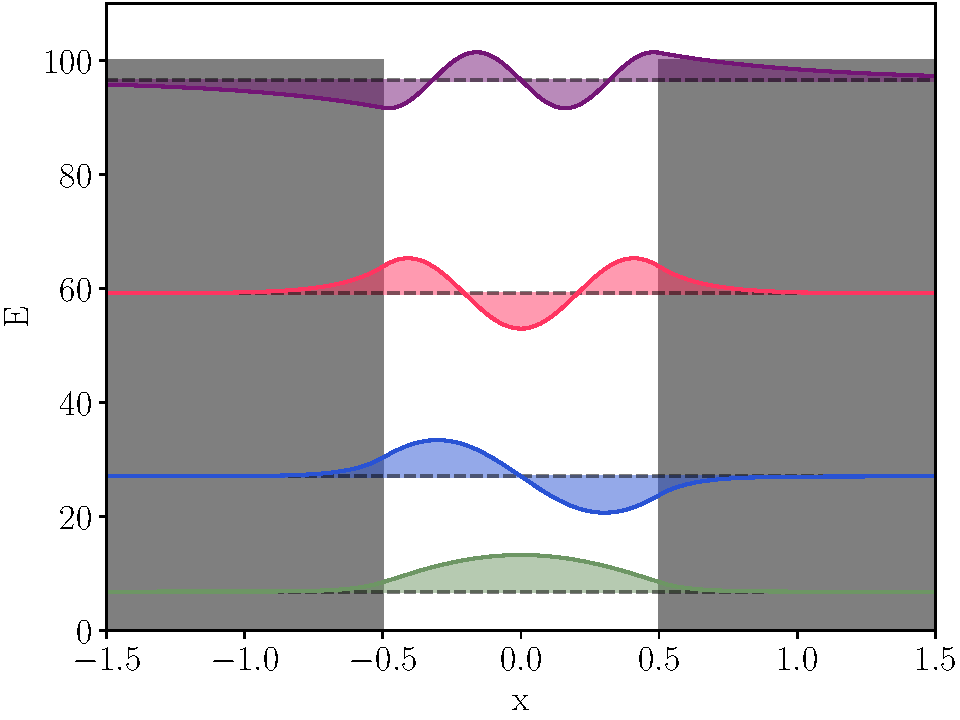
\includegraphics[width=0.7\textwidth]{finiteeigen.pdf}
	\caption{Prve 4 lastne funkcije končne potencialne jame globine 100 in širine 1 pomnoženih s 5}
\end{figure}
Bolj zahtevna je pri končni jami strelska metoda. Namreč pri njej robni pogoji niso tako preprosto poenostavljivi kot pri diferenčni. Iskane lastne funkcije potrebujemo ločiti na sode in lihe. Na primer za sode funkcije vzamemo da je $\psi(-\infty)=0$ in kot drugi robni pogoj postavimo, da mora biti odvod v $\psi'(0)=0$. Tako namreč dobimo v točki nič maksimum in posledično simetrično oziroma sodo funkcijo. 
Streljamo tako, da zadostimo robnemu pogoju v neskončnosti in nato iščemo energijo, ki bo zadostila robnemu pogoju v nič. Poglejmo si kako se odvod v točki nič obnaša v odvisnosti od energije.
\begin{figure}[H]
    \centering
    \begin{subfigure}[b]{0.49\textwidth}
        \centering
        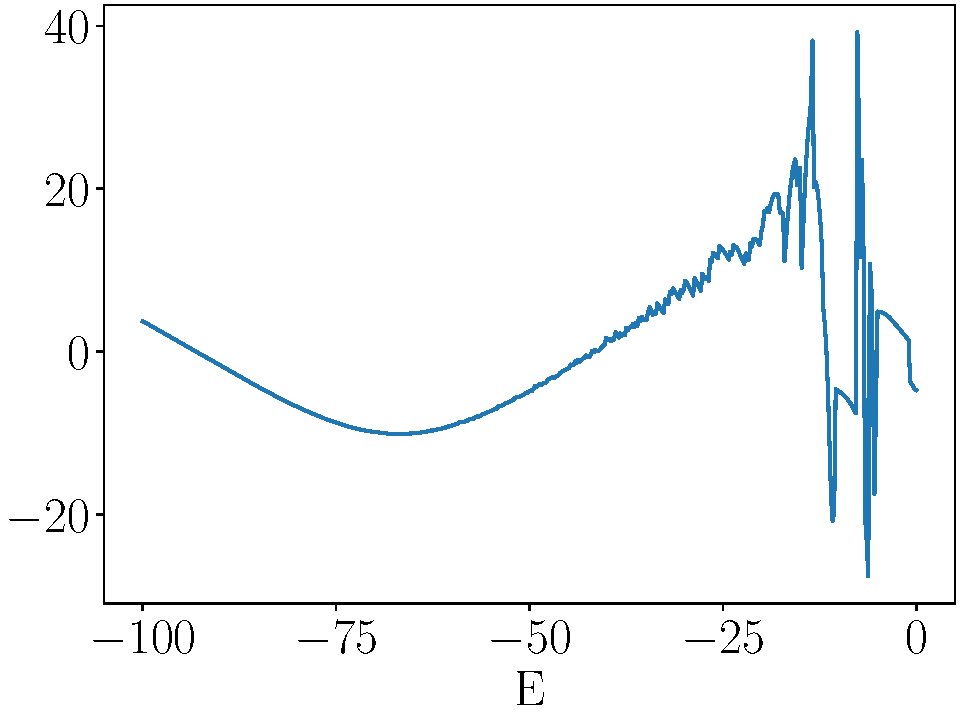
\includegraphics[width=\textwidth]{3oddaljenost.pdf}
		\caption{Robni pogoj $\psi(-3)=0$}
    \end{subfigure}
    \hfill
    \begin{subfigure}[b]{0.49\textwidth}
        \centering
		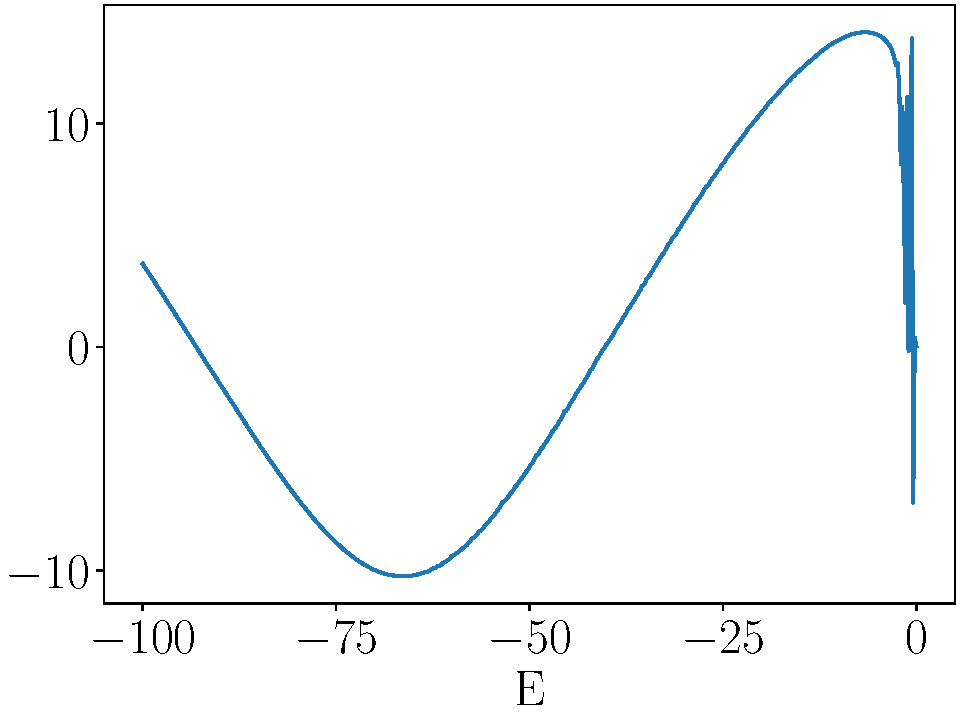
\includegraphics[width=\textwidth]{10oddaljenost.pdf}
        \caption{Robni pogoj $\psi(-10)=0$}
    \end{subfigure}
	\caption{Robni pogoj $\psi'(0)$ v odvisnosti od energije pri različni `neskončnosti`}
\end{figure}
Za numerično računanje seveda ne moremo uporabiti neskončnega intervala zato moramo izbrati primerno oddaljenost od roba potencialne jame, kjer ocenimo, da bo lastna funkcija dovolj konvergirala glede na našo toleranco. Z opazovanjem odvisnosti od energije najdemo lastni vrednosti, ki ustrezata prvim dvem lihim lastnim funkcijam. Ob energijah, ki ustrezajo rvišini potencialne jame pa opazimo precejšnjo nestabilnost, ki je zanimivo odvisna od tega kakšno vrednost smo izbrali kot `neskončno`.

\medskip

Poglavja o končni potencialni jami seveda ne moremo končati brez, da omenimo še njeno analitično rešitev. Sodo rešitev za jamo, ki je omejena na $|x|<\frac{a}{2}$ opišemo z naslednjim nastavkom
\begin{equation}
\psi(x) = \begin{cases} 
De^{-\kappa x}, & \frac{a}{2} < x \\
B\cos kx, & -\frac{a}{2} < x < \frac{a}{2} \\
\psi(-x), & x < -\frac{a}{2}
\end{cases}
\end{equation}
podobno lahko storimo za liho rešitev le, da izberemo namesto sode funkcije $\cos$ liho $\sin$ in rahlo drugače zapišemo simetrijo izven potencialne jame. Nato zapišemo robna pogoja za zveznost $D e^{-\kappa a/2}= B \cos{\frac{ka}{2}}$ in zvezno odvedljivost $-\kappa D e^{-\kappa a / 2} = - k B \sin{\frac{ka}{2}}$. S temi pogoji nato zapišemo transcedenčno enačbo $\kappa = k \tan{\frac{ka}{2}}$ katero s pomočjo zveze $p=\hbar k$ lahko preobrazimo v 
\begin{equation}
	z\tan{z} = \sqrt{z_0^2 - z^2}\text{,}
\end{equation}
kjer je $z = \frac{ka}{2}$ in $z_0=\frac{a}{2}\sqrt{\frac{2mV_0}{\hbar^2}}$. To enačbo najlažje rešimo numerično z iskanjem ničle. Konstante nato določimo s pomočjo normalizacije $\int^{\infty}_{-\infty}\psi^2=1$ in izraza za zveznost, ki smo ga zapisali že prej.
\section{Zaključek}
Naloga je sledila kot razširitev prejšnjih dveh nalog o reševanju diferencialnih enačb. Bila mi je precej zanimiva in tudi najverjetneje najtežja do sedaj, saj na videz preprosta implementacija to ni bila. Iz naloge sem se precej naučil in bom pridobljeno znanje gotovo še kdaj uporabil.
\end{document}
